
\begin{frame}
\frametitle{PQR: motivación}
Recordando...
\begin{itemize}
\item $\bf P$: Una posición en el dataset
\item \textbf{Q}: La posición obtenida a partir de aplicar el \enquote{mejor} movimiento a P, según el dataset
\item \textbf{R}: Una posición aleatoria obtenida a partir de P, tal que $R \neq Q$
\end{itemize}
\pause
Y los principios:
\begin{enumerate}
\item Si $P \rightarrow Q$, entonces $f(P)=-f(Q)$ (suma cero)
\item Si $P \rightarrow R$ tal que $R \neq Q$, entonces $f(R) > f(Q)$
\end{enumerate}
\end{frame}


\begin{frame}
\frametitle{PQR: motivación}
¿Los principios funcionan en la práctica? Veamos...
\begin{figure}
\centering
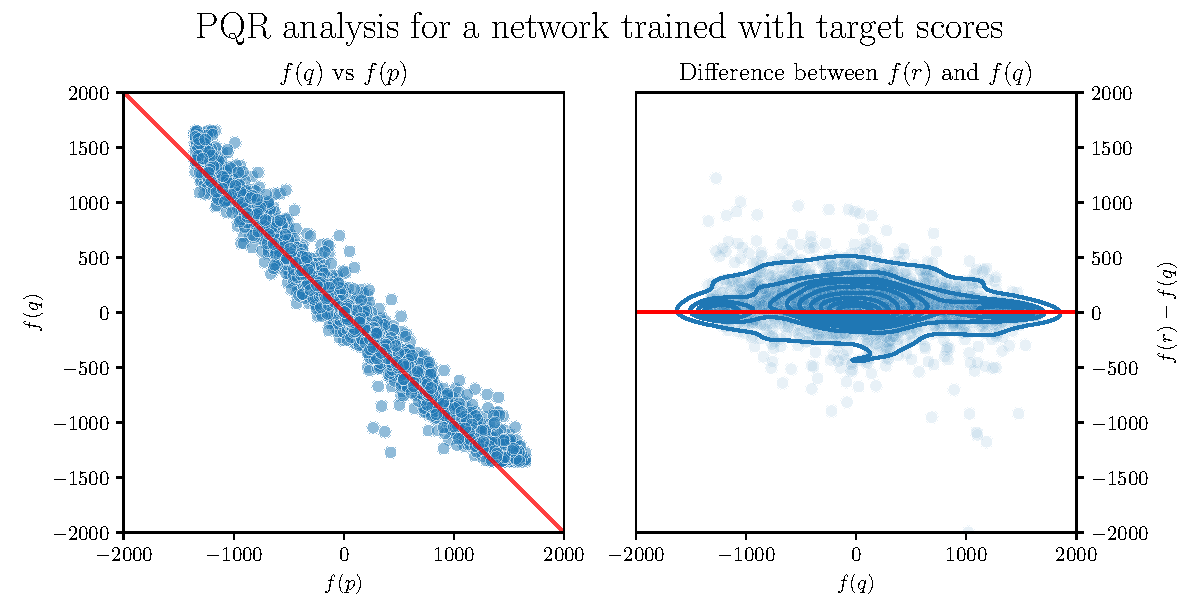
\includegraphics[width=\textwidth]{../thesis/dynamic/output/pqr_eval.pdf}
\caption{Analysis of $N=4000$ PQR samples using a model trained with target scores and the feature set \featureset{All}.}
\end{figure}
\end{frame}

\begin{frame}
\frametitle{PQR: experimento}
\begin{enumerate}[A.]
\item Entrenar de cero, directamente con PQR
\begin{itemize}
\item no espero que sea mejor que target scores
\end{itemize}
\pause
\item Continuar de un checkpoint entrenado con el otro método
\begin{itemize}
\item no tiene que aprender tanto de entrada
\item mejor caso: mejora lentamente
\item peor caso: se \enquote{olvida} todo lo anterior (resulta peor)
\item se entrena con distintos learning rates
\item (esto nunca se hizo antes)
\end{itemize}
\end{enumerate}
\end{frame}


\begin{frame}
\frametitle{PQR: experimento}
\textbf{Eligiendo} $\mathbf{R}$: más opciones para elegir $R$ $\Rightarrow$ es más probable que $R$ sea peor que $Q$.
\\
\pause
No podemos elegir un número fijo (por ejemplo, $> 10$) porque la cantidad de movimientos disponibles varía a lo largo de la partida.
\pause
\begin{figure}[H]
\centering
\makebox[0.78\textwidth]{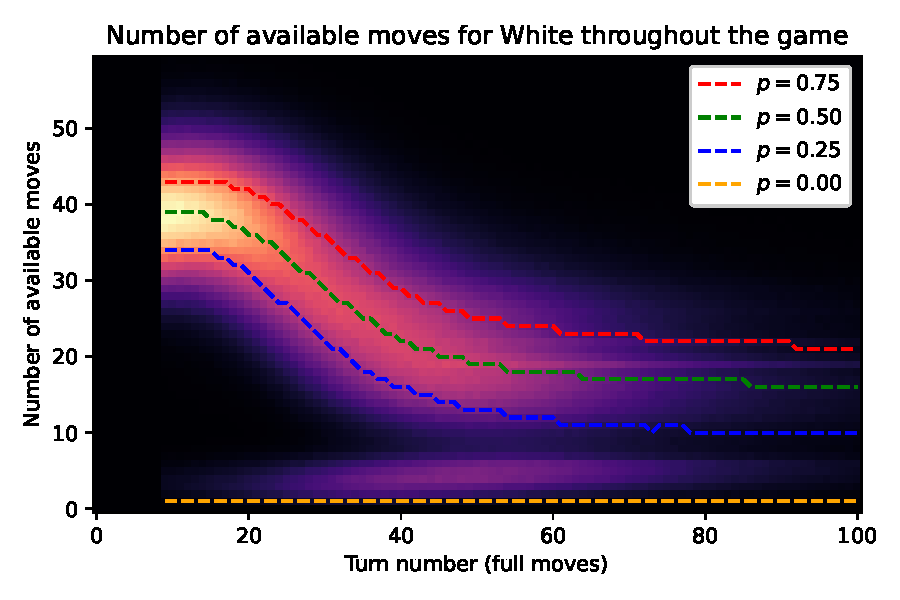
\includegraphics[width=0.78\textwidth]{../thesis/dynamic/output/avg_moves.pdf}}
\end{figure}
\end{frame}

\begin{frame}
\frametitle{PQR: resultados (A)}
\begin{figure}[H]
\centering
\makebox[\textwidth]{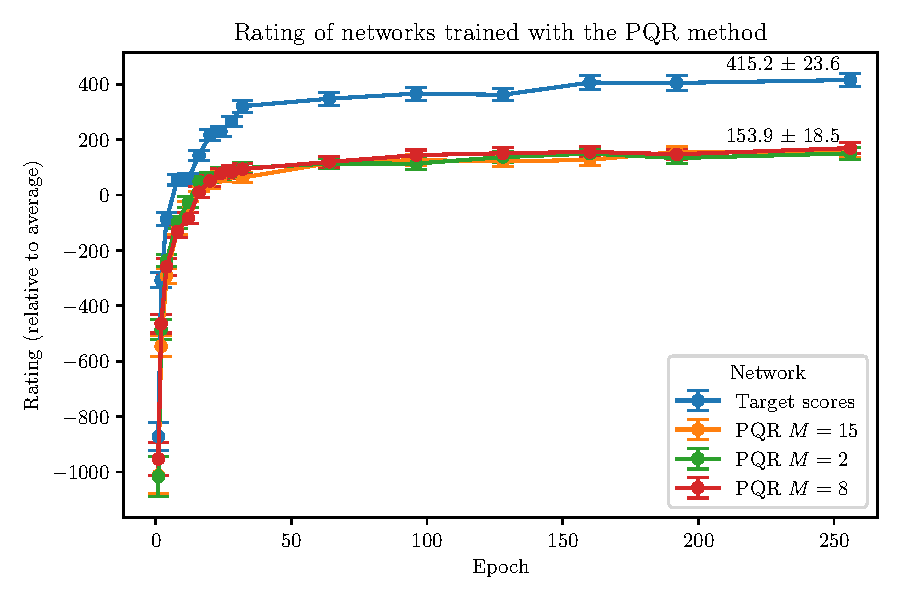
\includegraphics[width=\textwidth]{../thesis/dynamic/output/pqr_comparison.pdf}}
% \caption{Performance of networks trained from scratch using the PQR method varying the filtering parameter ($p=0,\ 0.25,\ 0.5,\ 0.75$). A network trained with target scores is shown for comparison.}
\end{figure}
\end{frame}


\begin{frame}
\frametitle{PQR: resultados (A)}
\begin{figure}[H]
\centering
\makebox[\textwidth]{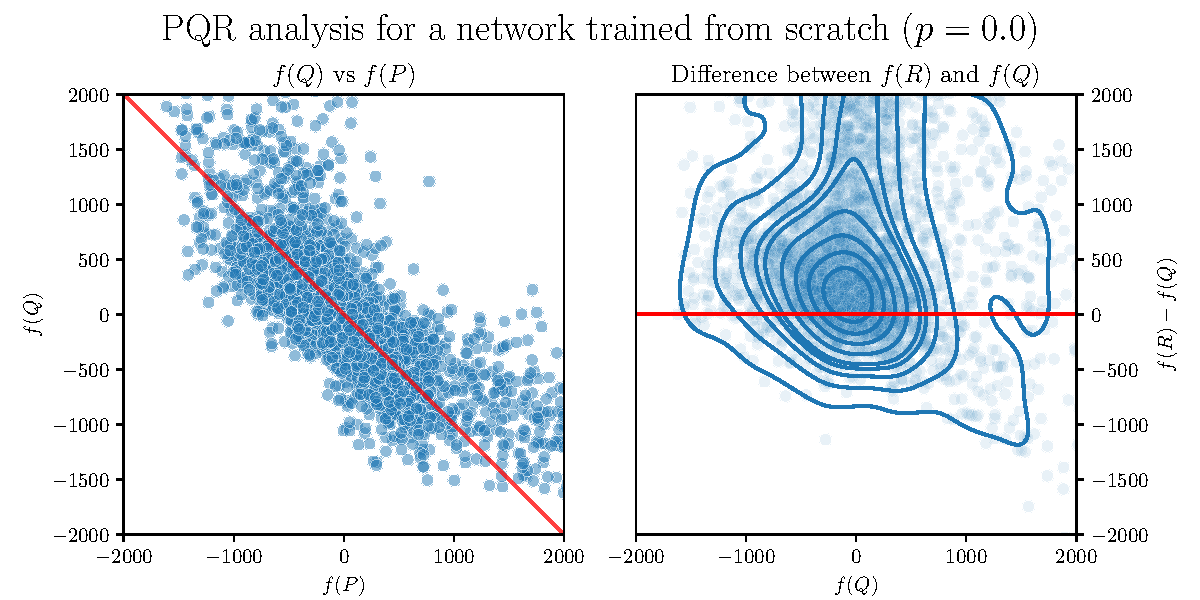
\includegraphics[width=\textwidth]{../thesis/dynamic/output/pqr_scratch.pdf}}
\caption{Analysis of $N=4000$ PQR samples using the epoch 256 of the model trained from scratch with no filtering ($p=0.0$) and the feature set \featureset{All}.}
\end{figure}
\end{frame}

\begin{frame}
\frametitle{PQR: resultados (B)}
\begin{figure}[H]
\centering
\makebox[\textwidth]{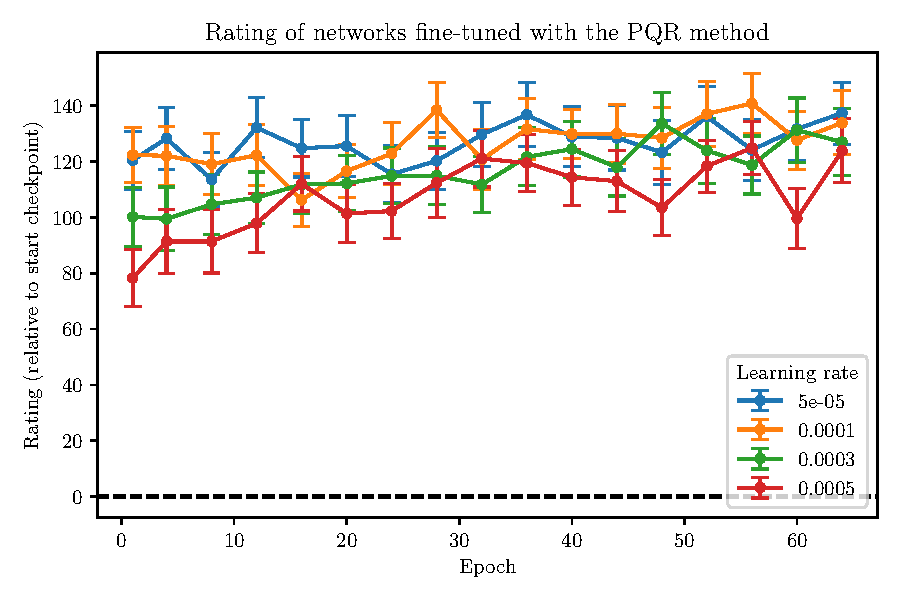
\includegraphics[width=\textwidth]{../thesis/dynamic/output/pqr_ckp.pdf}}
\end{figure}
\end{frame}
